\begin{IEEEbiography}[{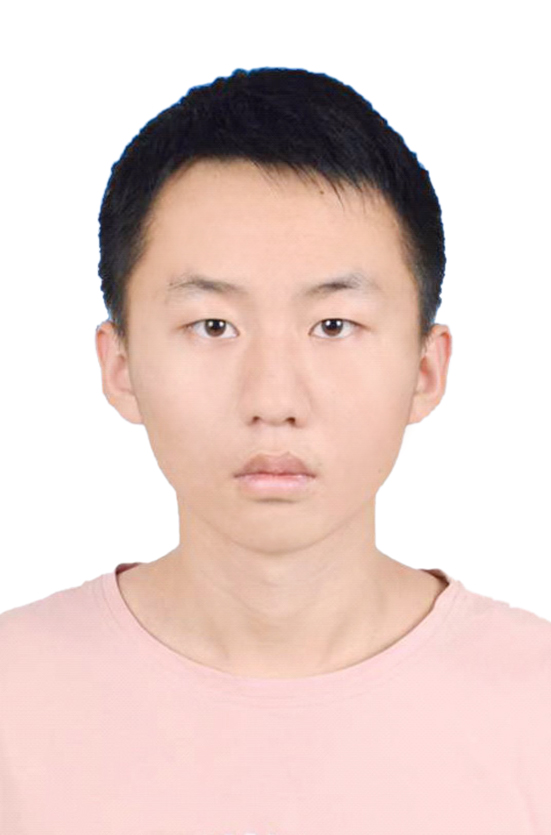
\includegraphics[width=1in,height=1.25in,clip,keepaspectratio]{assets/bio/yifei.jpg}}]{Yifei Gao} is pursuing the master degree at University College London. He previously obtained his B.Eng. degree from the College of Software Engineering at the University of Electronic Science and Technology of China in 2024. His current research interests encompass large language models, 3D reconstruction, and diffusion models.
\end{IEEEbiography}

\vspace{8pt}

\vspace{-33pt}

\begin{IEEEbiography}[{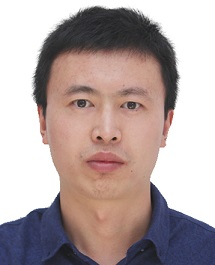
\includegraphics[width=1in,height=1.25in,clip,keepaspectratio]{assets/bio/leiwang.jpg}}]{Lei Wang} (Senior Member, IEEE) received the Ph.D. degree in Electrical Engineering from Xidian University, Xi'an, China, in 2010. From 2011 to 2012, he was with Huawei Technologies Company Ltd. From 2014 to 2015, he was with the Department of Embedded Systems Engineering, Incheon National University, as a Postdoctoral Fellow. He is currently an Associate Professor with the Shenzhen Institutes of Advanced Technology, Chinese Academy of Sciences, Shenzhen, China. He has authored or coauthored more than 70 papers in conferences and journals, including IEEE TRANSACTIONS ON CIRCUITS AND SYSTEMS FOR VIDEO TECHNOLOGY, IEEE TRANSACTIONS ON CYBERNETICS, IEEE TRANSACTIONS ON MULTIMEDIA, IEEE SIGNAL PROCESSING LETTERS, and NAACL. His research interests include image processing, transforms, machine learning, computer vision, 3-D reconstruction, and robotics.
\end{IEEEbiography}

\vspace{8pt}

\vspace{-33pt}

\begin{IEEEbiography}[{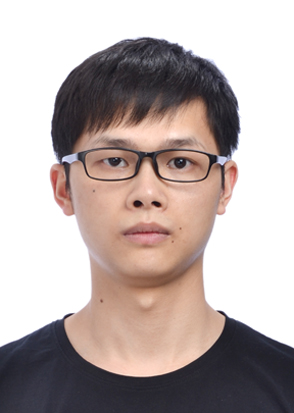
\includegraphics[width=1in,height=1.25in,clip,keepaspectratio]{assets/bio/rongcheng.jpg}}]{Rong-Cheng Tu}
received the B.S. degree in 2018 and the Ph.D. degree in 2023 from the Beijing Institute of Technology, Beijing, China. 
He is currently a Research Fellow with Nanyang Technological University (NTU), Singapore. 
His research interests include deep learning, information retrieval, and Large Language Model efficiency.
\end{IEEEbiography}

\vspace{8pt}

\vspace{-33pt}

\begin{IEEEbiography}[{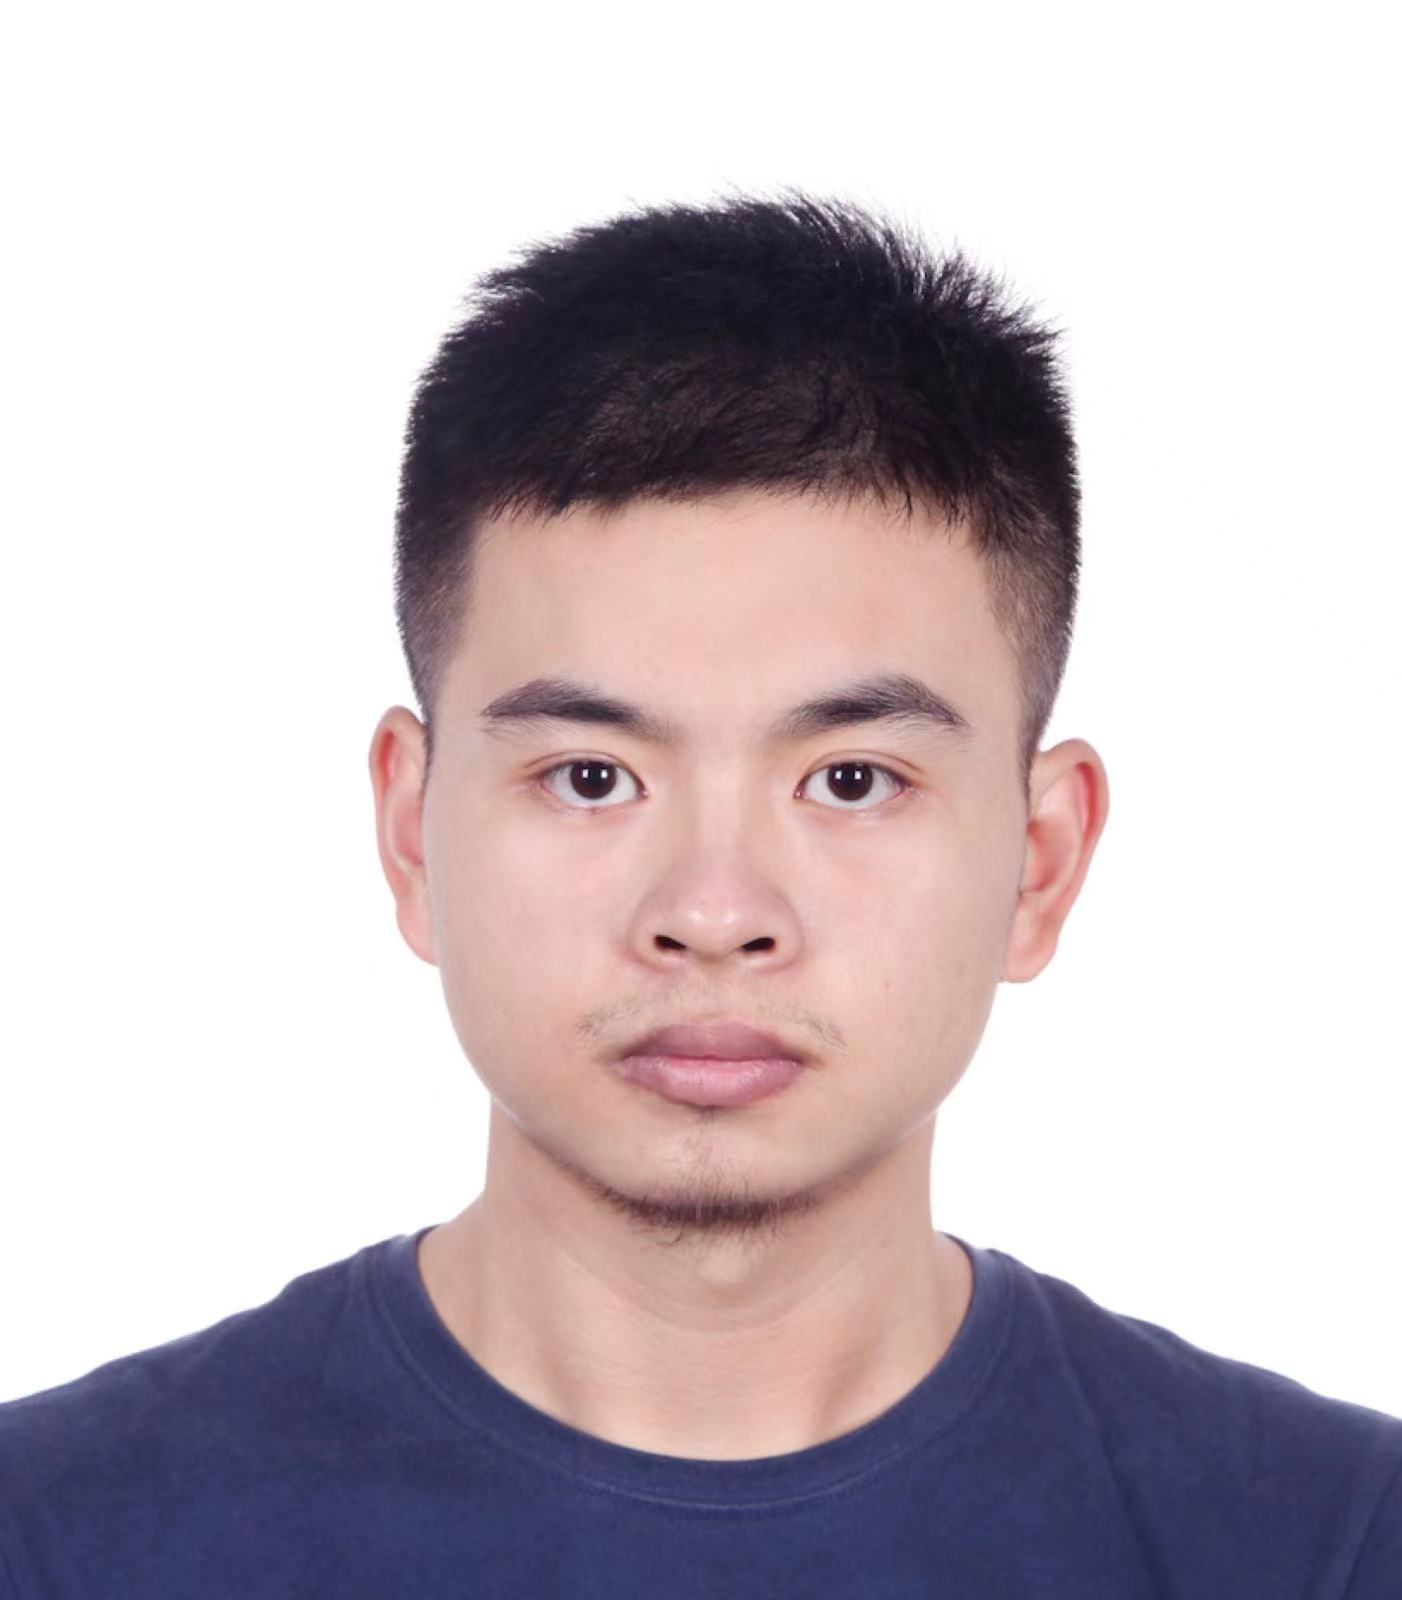
\includegraphics[width=1in,height=1.25in,clip,keepaspectratio]{assets/bio/qixin.jpg}}]{Qixin Zhang}
received his B.S. degree from the University of Science and Technology of China in 2018. He subsequently earned his Ph.D. degree in the School of Data Science at City University of Hong Kong in 2024. Currently, he is a Research Fellow at Nanyang Technological University, Singapore. His research interests include submodular optimization, subset selection and network prune. He has published over 15 papers in top data science venues such as ICML, NeurIPS, ICLR, AISTATS, AAAI and TKDE, etc.
\end{IEEEbiography}

\vspace{8pt}

\vspace{-33pt}

\begin{IEEEbiography}[{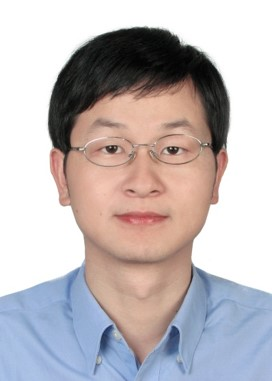
\includegraphics[width=1in,height=1.25in,clip,keepaspectratio]{assets/bio/juncheng.jpg}}]{Jun Cheng} (Senior Member, IEEE) received the B.Eng. and M.Eng. degrees from the University of Science and Technology of China, Hefei, China, in 1999 and 2002, respectively, and the Ph.D. degree from Chinese University of Hong Kong, Hong Kong, in 2006. He is currently a Professor with Shenzhen Institutes of Advanced Technology, Chinese Academy of Sciences, Shenzhen, China, where he is also the Director of the Laboratory for Human Machine Control. His current research interests include computer vision, robotics, machine intelligence, and control.
\end{IEEEbiography}

\vspace{8pt}

\vspace{-33pt}

\begin{IEEEbiography}[{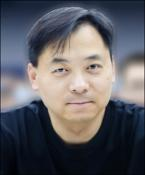
\includegraphics[width=1in,height=1.25in,clip,keepaspectratio]{assets/bio/dachengtao.jpeg}}]{Dacheng Tao} (F’15) is currently a Distinguished University Professor in the College of Computing \& Data Science at Nanyang Technological University. He mainly applies statistics and mathematics to artificial intelligence and data science, and his research is detailed in one monograph and over 200 publications in prestigious journals and proceedings at leading conferences, with best paper awards, best student paper awards, and test-of-time awards. His publications have been cited over 126K times and he has an hindex 160+ in Google Scholar. He received the 2015 and 2020 Australian Eureka Prize, the 2018 IEEE ICDM Research Contributions Award, and the 2021 IEEE Computer Society McCluskey Technical Achievement Award. He is a Fellow of the Australian Academy of Science, AAAS, ACM and IEEE.
\end{IEEEbiography}